\chapter{Kiến thức cơ sở}\label{chap2}
Trước khi đi sâu hơn về giải pháp kiểm thử đơn vị tự động cho mã nguồn C/C++ chứa hàm thiếu định nghĩa, chương này sẽ trình bày một số kiến thức cơ bản, quan trọng liên quan đến đề tài, tạo nền tảng cho việc hiểu rõ hơn về các khái niệm và phương pháp được đề cập trong khóa luận. Trước hết, khóa luận trình bày một số khái niệm, thuật ngữ liên quan đến kĩ thuật kiểm thử dòng điều khiển trong kiểm thử phần mềm. Tiếp theo, khóa luận chia sẻ chi tiết hơn về kĩ thuật kiểm thử tượng trưng động và làm rõ cơ chế sinh dữ liệu kiểm thử từ tập ràng buộc. Cuối cùng, khóa luận trình bày một số khái niệm liên quan đến hàm thiếu định nghĩa và mô tả tổng quan phương pháp sinh stub tự động.

\section{Một số khái niệm, thuật ngữ trong kiểm thử dòng điều khiển}
\subsection{Cây cú pháp trừu tượng và đồ thị dòng điều khiển} \label{sec:kno-ast-and-cfg}
Cây cú pháp trừu tượng (Abstract Syntax Tree - AST) là một biểu diễn cấu trúc cú pháp của một đoạn mã nguồn. AST được tạo ra từ quá trình phân tích cú pháp của ngôn ngữ lập trình và thường được sử dụng trong các bước biên dịch và xử lý ngôn ngữ. Về cơ bản, AST là một cách biểu diễn khác của mã nguồn mà trong đó, thay vì dạng văn bản thuần túy, các thành phần mã nguồn sẽ được thể hiện bằng từng thành phần trong cây. Việc sử dụng cây cú pháp trừu tượng trong kiểm thử tự động cho phép ta dễ dàng lấy ra các thông tin cần thiết thay vì phân tích mã nguồn từ dạng văn bản.
	
Đồ thị dòng điều khiển (Control Flow Graph - CFG) đóng vai trò quan trọng trong phương pháp kiểm thử dòng điều khiển bởi phương pháp này đều có mục tiêu viếng thăm tối đa các đỉnh trên đồ thị. Đồ thị dòng điều khiển có thể được xây dựng dễ dàng từ AST của mã nguồn. Đồ thị dòng điều khiển được định nghĩa như Định nghĩa 2.1.

\textbf{Định nghĩa 2.1}: Đồ thị dòng điều khiển là một đồ thị có hướng gồm các điểm tương ứng với các câu lệnh/nhóm câu lệnh và các cạnh là các dòng điều khiển giữa các câu lệnh/nhóm câu lệnh. Nếu $i$ và $j$ là các điểm của đồ thị dòng điều khiển thì tồn tại một cạnh từ $i$ đến $j$ nếu lệnh tương ứng với $j$ có thể được thực hiện ngay sau lệnh tương ứng với $i$~\cite{GiaoTrinhKiemThu}.

Đồ thị dòng điều khiển bao gồm các thành phần chính là điểm xuất phát, khối xử lý, điểm quyết định, điểm nối và điểm kết thúc. Các thành phần cơ bản trong đồ thị dòng điều khiển được mô tả trong Hình \ref{fig:flow-element}. Các cấu trúc điều khiển cơ bản như tuần tự, rẽ nhánh, switch, vòng lặp while-do và do-while trong ngôn ngữ C/C++ được mô phỏng dưới dạng các thành phần cơ bản của CFG như Hình \ref{fig:flow-structure}.
\begin{figure}[h]
	\centering
	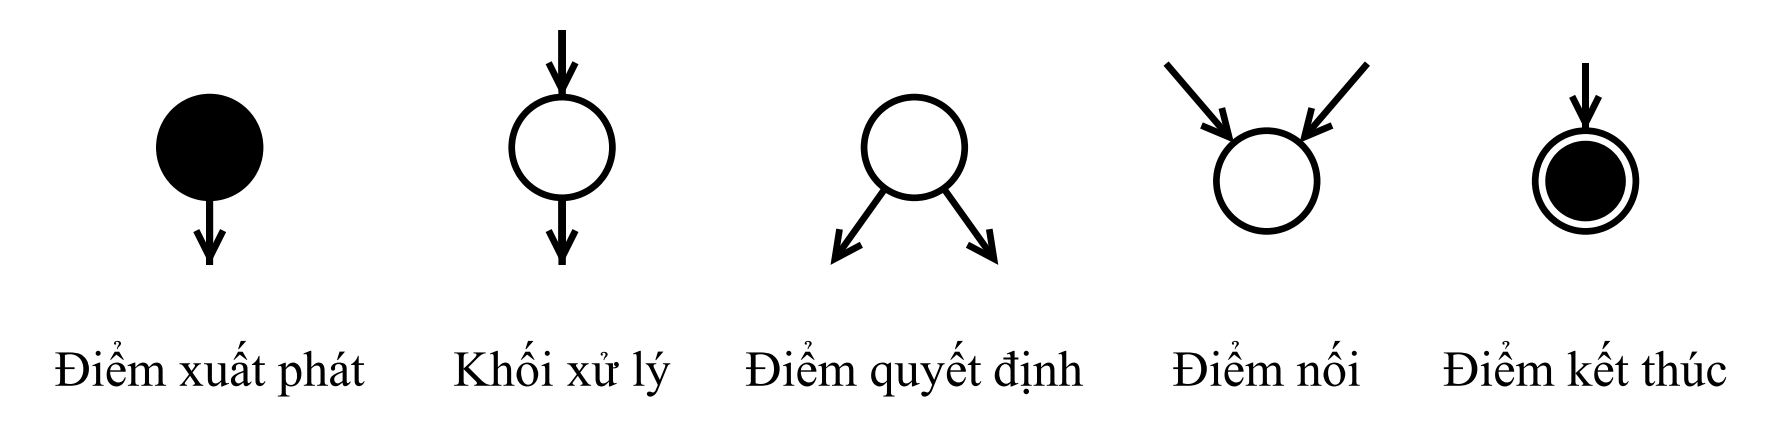
\includegraphics[width=\linewidth]{images/flow-element.png}
	\caption{Các thành phần cơ bản trong đồ thị dòng điều khiển \cite{GiaoTrinhKiemThu}.}
	\label{fig:flow-element}
\end{figure}

\begin{figure}[h]
	\centering
	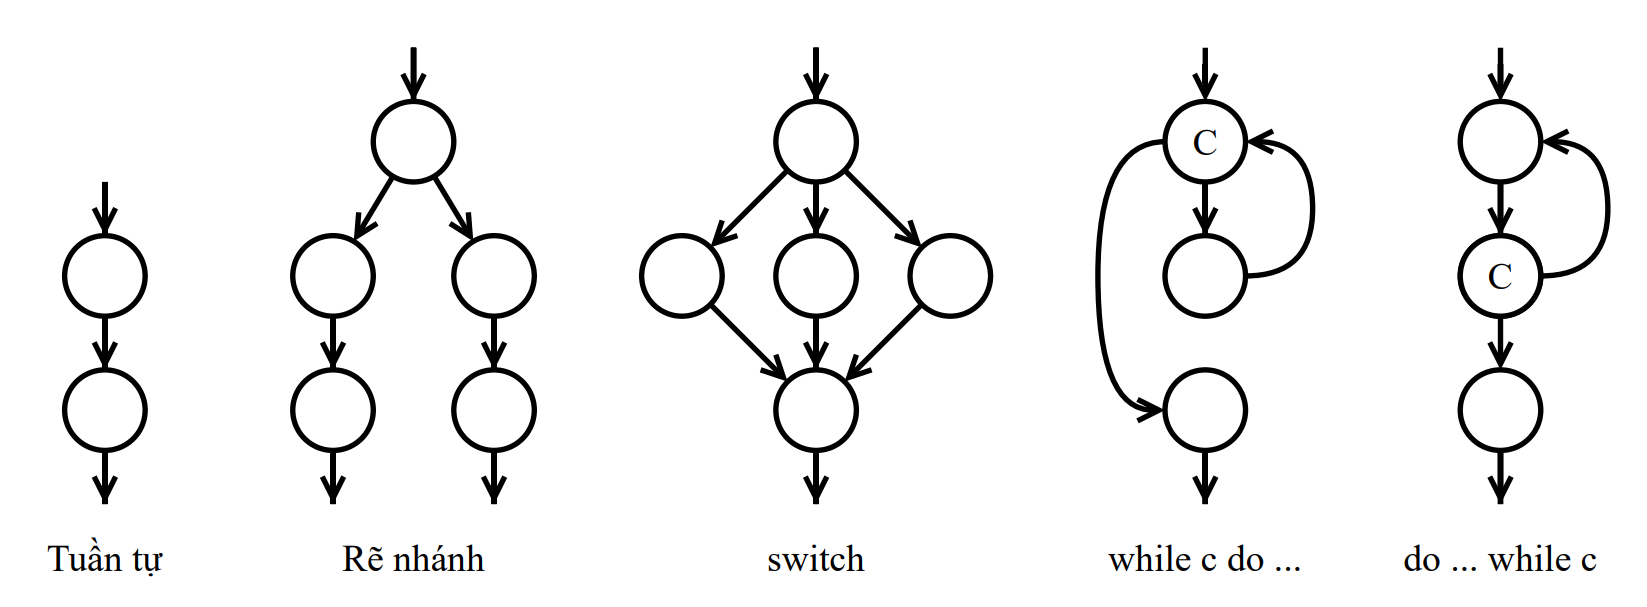
\includegraphics[width=\linewidth]{images/flow-structure.png}
	\caption{Các cấu trúc điều khiển phổ biến trong dồ thị dòng điều khiển \cite{GiaoTrinhKiemThu}.}
	\label{fig:flow-structure}
\end{figure}

\subsection{Đường thi hành}\label{sec:path}
Đường thi hành là một tập hợp có thứ tự các đỉnh trên CFG thể hiện thứ tự viếng thăm khi thực thi đơn vị kiểm thử tương ứng. Nói cách khác, đường thi hành biểu diễn các câu lệnh được chạy khi thực thi đơn vị kiểm thử với một bộ tham số đầu vào. Định nghĩa chính xác của đường thi hành như Định nghĩa 2.2.

\textbf{Định nghĩa 2.2}: Đường thi hành là một đường đi từ điểm xuất phát đến điểm kết thúc của CFG, được biểu diễn bằng tập hợp các điểm từ $v_1$ đến $v_n$ sao cho cứ hai điểm cạnh nhau thì có cạnh nối theo hướng từ trái qua phải. Nếu cạnh ($v_i$, $v_j$) là nhánh sai thì biểu thức điều kiện tại điểm $v_i$ được viết dưới dạng phủ định $!v_i$~\cite{GiaoTrinhKiemThu}.

Đường thi hành có thể chứa rất nhiều câu lệnh và rất nhiều nhánh điều kiện. Điều này dẫn tới việc một đơn vị kiểm thử có thể chứa đường thi hành không khả thi và có thể bùng nổ số lượng đường thi hành. Một đường thi hành không khả thi khi tồn tại những điều kiện không thể thỏa mãn được. Một ví dụ có thể kể đến đó là câu lệnh so sánh \tcode{if(0~==~1)}. Phép so sánh này không bao giờ đúng nên các đỉnh CFG trong nhánh đúng của đỉnh so sánh trên sẽ không thể viếng thăm. Về khả năng bùng nổ số lượng đường thi hành, điều này có thể thấy rõ thông qua các vòng lặp. Các vòng lặp với số lần lặp chưa biết trước có thể tạo ra vô số đường thi hành. Vì vậy việc kiểm thử toàn bộ đường thi hành là một thách thức lớn.

Như vậy, việc sinh dữ liệu kiểm thử cho một đường thi hành tương ứng với quá trình tìm giá trị bộ tham số đầu vào sao cho viếng thăm được toàn bộ đỉnh trên đường thi hành. Trong thực tế, số lượng đường thi hành của một đơn vị kiểm thử có thể rất lớn. Do vậy, việc lựa chọn tập đường thi hành sao cho đạt độ phủ mã nguồn yêu cầu là một thách thức lớn.

\subsection{Độ phủ mã nguồn} \label{sec:coverage}
Độ phủ mã nguồn là một đơn vị đo số lượng thành phần trong đơn vị kiểm thử được viếng thăm bởi bộ dữ liệu tham số đầu vào. Các thành phần liên quan có thể là câu lệnh, điểm quyết định, điều kiện con, đường thi hành hay là sự kết hợp của chúng \cite{GiaoTrinhKiemThu}. Bộ kiểm thử có độ tin cậy càng cao khi độ phủ đơn vị kiểm thử càng lớn. Ba loại độ phủ mã nguồn được sử dụng phổ biến trong thực tế gồm $C_1$, $C_2$ và $C_3$~\cite{GiaoTrinhKiemThu}. Một số tác giả sử dụng các khái niệm tương ứng gồm Statement, Branch và MCDC (Modified Condition/Decision Coverage). Khóa luận sử dụng khái niệm $C_1$, $C_2$ và $C_3$ với định nghĩa như sau:
\begin{itemize}
	\item Độ phủ $C_1$: Được hiểu là độ phủ ở mức câu lệnh, tức mỗi câu lệnh trong đơn vị kiểm thử được thực thi ít nhất một lần sau khi chạy tập ca kiểm thử.
	
	\item Độ phủ $C_2$: Được hiểu là độ phủ ở mức điểm quyết định, tức mỗi điểm quyết định trong CFG của đơn vị kiểm thử đều được thực hiện ít nhất một lần cả nhánh đúng và sai sau khi chạy tập ca kiểm thử.
	
	\item Độ phủ $C_3$: Là độ phủ có điều kiện chặt nhất trong ba loại độ phủ. Điều kiện để đảm bảo độ đo này là các điều kiện con thuộc các điều kiện phức tạp tương ứng với các điểm quyết định trong đồ thị dòng điều khiển của đơn vị cần kiểm thử đều được thực hiện ít nhất một lần cả hai nhánh đúng và sai. Với các phần mềm yêu cầu tính đúng đắn cao, việc sử dụng độ đo $C_3$ để đánh giá mã nguồn là cần thiết.
\end{itemize}

\section{Kiểm thử tượng trưng động}
Như đã đề cập ở Chương \nameref{chap1}, kiểm thử tượng trưng động là kĩ thuật kiểm thử áp dụng đồng thời kiểm thử tĩnh và kiểm thử động với ba pha chính là sinh dữ liệu kiểm thử ngẫu nhiên, thực thi ca kiểm thử \& phân tích đường thi hành và sinh dữ liệu kiểm thử có định hướng. Trong pha đầu tiên, một số dữ liệu kiểm thử được sinh ngẫu nhiên. Các dữ liệu kiểm thử sau đó được thực thi trong pha thứ hai. Nhờ việc thực thi các dữ liệu kiểm thử khởi tạo, kiểm thử tượng trưng động xác định được tập các điểm chưa được viếng thăm và
tìm kiếm đường thi hành từ điểm xuất phát đến điểm đó. Một số nhà nghiên cứu lựa chọn đường thi hành ngắn nhất tới một điểm chưa viếng thăm nhằm tối ưu hóa số lượng ca kiểm thử như SDART~\cite{SDART}. Nếu tìm được đường thi hành chưa được viếng thăm, pha thứ ba chuyển đổi đường thi hành thành các ràng buộc sử dụng kỹ thuật thực thi giá trị tượng trưng~\cite{SymbolicExecutionForSoftwareTestingThreeDecadesLater}. Các ràng buộc được biểu diễn dưới dạng biểu thức logic và được chuyển đổi thành đầu vào của bộ giải hệ ràng buộc. Cuối cùng, bộ giải hệ ràng buộc chịu trách nhiệm giải các ràng buộc và cho ra được một nghiệm - dữ liệu kiểm thử mới. Quá trình sinh dữ liệu kiểm thử sau đó lặp lại từ pha thứ hai cho đến khi tất cả đỉnh trong CFG đã được thăm hoặc chương trình chạy quá thời gian quy định. 

Kỹ thuật kiểm thử tượng trưng động có khả năng đạt độ phủ cao hơn bởi khả năng sinh dữ liệu có hướng dựa trên ràng buộc của đường thi hành. Tập ràng buộc là tập các điều kiện tạo ra bởi tập các kiểm quyết định khi áp dụng kỹ thuật thực thi tượng trưng trên một đường thi hành. Nói cách khác, tập ràng buộc chứa các điều kiện mà dữ liệu đầu vào cần thỏa mãn để ca kiểm thử phủ đường thi hành mong muốn. Dữ liệu đầu vào như vậy được gọi là dữ liệu kiểm thử có hướng. Dữ liệu kiểm thử có hướng cho mỗi đường thi hành có thể thu được bằng cách giải hệ ràng buộc. Trong đó, giải hệ ràng buộc là việc tìm nghiệm cho một tập các ràng buộc, biểu diễn bởi các phép toán điều kiện, sao cho với các giá trị biến đầu vào trong nghiệm thì tất cả các ràng buộc được thỏa mãn~\cite{ref-constraints}. Hiện nay, có nhiều thư viện và công cụ hỗ trợ giải hệ ràng buộc trong đó nổi bật là bộ giải Z3\footnote{https://github.com/Z3Prover/z3}.

Bộ giải Z3 là một công cụ được phát triển bởi Nhóm Nghiên cứu về Kỹ thuật Phần mềm (RiSE) tại Microsoft Research. Được xây dựng chủ yếu bằng ngôn ngữ C++, Z3 hỗ trợ giải hệ ràng buộc của nhiều loại dữ liệu như số nguyên, số thực, mảng, hàm tượng trưng, vectơ bit, và các biểu thức số học khác nhau. Z3 được thiết kế để hỗ trợ định dạng SMT-LIB\footnote{http://smtlib.github.io/jSMTLIB/SMTLIBTutorial.pdf}, một định dạng tiêu chuẩn sử dụng để giải quyết các vấn đề liên quan đến giải ràng buộc. Để sử dụng bộ giải, hệ ràng buộc cần được biểu diễn dưới định dạng SMT-LIB và lưu trữ trong tệp *.smt2. Cấu trúc của tệp này bao gồm ba phần chính: phần khai báo, phần định nghĩa ràng buộc và phần tiện ích. Phần khai báo đầu tiên trong tệp là nơi các biến trong hệ ràng buộc được khai báo theo cú pháp SMT-LIB. Sau đó, các ràng buộc được thêm vào bằng cách sử dụng lệnh assert. Cuối cùng, phần tiện ích cung cấp các cú pháp sẵn có để người dùng thực hiện các thao tác như đặt thời gian giải quyết tối đa, xác định mô hình giải ràng buộc, và nhiều tính năng khác.

\section{Hàm thiếu định nghĩa} \label{sec:kno-undefine}
\subsection{Tổng quan về hàm thiếu định nghĩa}
Như đã đề cập ở Chương~\nameref{chap1}, hàm thiếu định nghĩa là những hàm mà có nguyên mẫu được khai báo, nhưng không có thân hàm (định nghĩa hàm). Để làm rõ hơn khái niệm này, ta cần hiểu thêm về cách khai báo hàm trong ngôn ngữ C/C++. Về cơ bản, một hàm gồm hai phần chính đó là nguyên mẫu hàm và thân hàm. Trong đó, nguyên mẫu hàm thông báo cho trình biên dịch biết tên hàm, kiểu trả về của hàm và danh sách tham số mà hàm nhận. Thân hàm là phần nội dung của hàm nằm trong cặp ngoặc \tcode{\{\}}. Ngôn ngữ C/C++ cung cấp hai cách để người dùng khai báo một hàm (ngoại trừ hàm lambda) gồm khai báo đầy đủ và khai báo tách rời.
\vspace{5mm}
\begin{lstlisting}[language=C++, captionpos=b, caption={Ví dụ về khai báo hàm đầy đủ và khai báo hàm tách rời.}, label={cod:kno-undef}]
// Full function declaration
int foo(int a, int b) { return a + b; }
// Function prototype + Function defintion 
int bar(int a, int b);
int echo(double);
int main() { bar(1,2); }
int bar(int a, int b) { return a - b; }
\end{lstlisting}

Đoạn mã \ref{cod:kno-undef} minh họa ví dụ về khai báo đầy đủ và khai báo tách rời. Dòng~1-3 thể hiện khai báo tách rời của hàm~\tcode{foo} với nguyên mẫu hàm và thân hàm đều nằm trong cùng một câu lệnh khai báo. Dòng~6 thể hiện khai báo nguyên mẫu hàm của hàm~\tcode{bar} và cho biết hàm này trả về giá trị kiểu \tcode{int} và nhận hai tham số đầu vào kiểu \tcode{int}. Dòng~7 cũng thể hiện nguyên mẫu hàm \tcode{echo}. Dòng~11-13 thể hiện khai báo định nghĩa hàm (thân hàm) của hàm \tcode{bar}.

Nguyên mẫu hàm là một trong những tính năng quan trọng của ngôn ngữ C/C++. Nguyên mẫu hàm cung cấp cho trình biên dịch biết những thông tin cơ bản của hàm và trình biên dịch ngầm hiểu rằng định nghĩa của hàm này có tồn tại. Cơ chế này giúp tăng tính tái sử dụng mã nguồn trong ngôn ngữ C/C++ bởi người dùng có thể tái sử dụng các nguyên mẫu hàm trong tệp header mà không cần biết nội dung chi tiết trong hàm đó.

Nguyên mẫu hàm là một tính năng hữu ích song nó cũng có nhược điểm. Nhược điểm của tính năng này đó là sự phụ thuộc vào người dùng. Một nguyên mẫu hàm không cần thiết phải có định nghĩa hàm bởi có thể nó không được sử dụng trong mã nguồn. Với ví dụ trong Đoạn mã~\ref{cod:kno-undef}, nguyên mẫu hàm \tcode{echo} không cần có định nghĩa bởi nó không được sử dụng trong bất kì thành phần nào khác. Trình biên dịch có khả năng tự xác định các nguyên mẫu hàm được sử dụng khi phân tích cú pháp mã nguồn ở bước biên dịch. Quá trình liên kết các tệp đối tượng có mục đích xác định định nghĩa hàm tương ứng với từng nguyên mẫu hàm. Ở bước này, nếu trình biên dịch không thể tìm thấy định nghĩa hàm tương ứng, nguyên mẫu hàm được coi là hàm thiếu định nghĩa.
\subsection{Nguyên mẫu hàm ảo và lỗi thiếu bảng ký hiệu ảo}
Hàm ảo là một cơ chế mới được giới thiệu trong ngôn ngữ C++ nhằm thể hiện các đặc trưng hướng đối tượng so với ngôn ngữ C. Hàm ảo là một hàm đặc biệt, chỉ có thể khai báo trong lớp và có khả năng ghi đè bởi hàm ở lớp dẫn xuất. Khi hàm ảo ở lớp cơ sở được gọi, chương trình sẽ tự động hiểu và chọn đúng đối tượng ở lớp dẫn xuất để gọi đúng hàm ghi đè. Khả năng trên được gọi là đa hình. Nguyên mẫu hàm ảo cũng có các đặc điểm tương tự như nguyên mẫu hàm cơ bản.

Để có được khả năng đa hình, ngôn ngữ C++ giới thiệu một khái niệm mới có tên là bảng ký hiệu ảo (Vtable). Vtable là bảng lưu trữ các khai báo biến, hàm có trong một kiểu dữ liệu tự định nghĩa do trình biên dịch tạo ra khi biên dịch một tệp mã nguồn. Vtable là công cụ giúp trình biên dịch biết một biến đã được định nghĩa hay chưa, biến đó thuộc kiểu gì, từ đó thông báo đến người dùng nếu có lỗi ngữ pháp. Vtable còn là công cụ giúp chương trình xác định được hàm nào sẽ được thực thi bằng cách sử dụng cơ chế liên kết động. Nếu hàm ảo, thuần ảo thiếu định nghĩa hàm thì khi liên kết, trình biên dịch sẽ báo lỗi do không biết chương trình sẽ cần hàm nào để chạy. Khác với các nguyên mẫu hàm cơ bản, trình biên dịch không hiển thị lỗi hàm thiếu định nghĩa nếu không tìm thấy định nghĩa của hàm ảo mà sẽ hiển thị lỗi thiếu bảng ký hiệu ảo. Nguyên nhân gây ra lỗi này là bởi trình biên dịch không cho phép gọi hàm ảo nếu nó không có ít nhất một hàm ghi đè.\\

\begin{lstlisting}[language=C++, captionpos=b, caption={Ví dụ về lỗi thiếu bảng ký hiệu ảo.}, label={cod:kno-vtable}]
	class A {
		virtual int echo() {}
		virtual int foo();
		virtual int bar();
	};
	class B : public A {
		int bar() {}
	}
\end{lstlisting}

Để làm rõ hơn ví dụ về lỗi thiếu bảng ký hiệu ảo, ta xét ví dụ trong Đoạn mã~\ref{cod:kno-vtable}. Đoạn mã này chứa hai lớp \tcode{A} và \tcode{B} trong đó \tcode{B} là lớp dẫn xuất của \tcode{A}. Lớp \tcode{A} có chứa ba nguyên mẫu hàm ảo, trong đó hàm~\tcode{bar} được ghi đè ở lớp dẫn xuât và hàm~\tcode{echo} là khai báo hàm ảo đầy đủ. Trong quá trình liên kết để tạo thành tệp thực thi, trình biên dịch báo lỗi thiếu Vtable cho kiểu \tcode{A} bởi trình biên dịch không thể tìm thấy hàm ghi đè nguyên mẫu hàm ảo \tcode{foo} ở lớp dẫn xuất.

\subsection{Vai trò trong các dự án C/C++}
Kể từ khi được giới thiệu trong ngôn ngữ C, nguyên mẫu hàm đóng vai trò quan trọng các dự án C/C++ và được sử dụng phổ biến trong quá trình phát triển phần mềm.	Về mặt kỹ thuật, nguyên mẫu hàm giúp tạo ra một bản thiết kế cho các hàm trước khi chúng được triển khai. Điều này giúp kiểm soát việc sử dụng hàm, đồng thời cung cấp thông tin đầy đủ cho trình biên dịch để kiểm tra tính đúng đắn của mã nguồn. Về mặt phát triển, nguyên mẫu hàm cho phép các thành viên trong nhóm phát triển đặt ra những lớp giao diện, các hành vi sẽ được cung cấp bởi mô-đun họ phụ trách. Điều này thúc đẩy quá trình phát triển phần mềm nhanh hơn bởi các thành viên không cần phải đợi sự hoàn thiện từ các thành phần phụ thuộc. 

Trong ngôn ngữ C++, vai trò của nguyên mẫu hàm được bổ sung trong đặc trưng kế thừa và đa hình với nguyên mẫu hàm ảo. Khi một lớp cơ sở chứa một hàm ảo, các lớp kế thừa có thể cung cấp triển khai riêng của hàm đó mà không cần thay đổi nguyên mẫu. Điều này tạo điều kiện cho việc chia sẻ chức năng giữa các lớp và giúp tăng tính linh hoạt của hệ thống. Nguyên mẫu hàm ảo tạo ra khả năng đa hình, cho phép gọi hàm dựa trên kiểu đối tượng thực tế thay vì kiểu của biến con trỏ hay tham chiếu. Điều này làm cho mã nguồn trở nên linh hoạt và dễ bảo trì, đặc biệt là trong các hệ thống lớn với nhiều lớp và đối tượng.

Do quá trình kiểm thử đơn vị diễn ra song song với quá trình phát triển nên ta không thể tránh khỏi tình trạng mã nguồn tồn tại một số nguyên mẫu hàm thiếu định nghĩa. Vì vậy, nhu cầu phát triển một giải pháp kiểm thử tự động đặc biệt cho mã nguồn C/C++ chứa hàm thiếu định nghĩa là vô cùng thiết yếu. Theo khảo sát của khóa luận về phương pháp xử lý hàm thiếu định nghĩa, hiện chưa có phương pháp nào được đề xuất vậy nên khóa luận sẽ thảo luận chi tiết về phương pháp giải quyết ở Chương~\ref{chap3}.

\section{Sinh giả lập mã nguồn tự động} \label{sec:autostub-Lam}
Trong quá trình phát triển phần mềm, hai giai đoạn quan trọng là cài đặt và kiểm thử thường diễn ra đồng thời để giảm thiểu thời gian phát triển và đồng thời đảm bảo chất lượng sản phẩm. Tuy nhiên, điều này có thể dẫn đến việc mã nguồn kiểm thử chứa các thành phần chưa hoàn thiện. Điều này đặt ra thách thức khi đơn vị kiểm thử có thể chứa các lời gọi hàm chưa được đầy đủ, ảnh hưởng đến quá trình kiểm thử chính xác và hiệu quả.

Một số phương pháp sinh stub tự động đã được đề xuất để giải quyết bài toán trên. Trong đó, năm 2022, ông Trần Nguyên Hương và các cộng sự đã đề xuất phương pháp AS4UT~\cite{TUNG2022106821} giúp sinh stub tự động, sử dụng trong kiểm thử đơn vị các dự án C/C++. Ý tưởng chính của phương pháp là xem mỗi lời gọi hàm như một biến giả. Giai đoạn tiền xử lý CFG được thêm vào hướng tiếp cận kiểm thử tượng trưng động. Trong giai đoạn này, mọi lời gọi hàm trong CFG của đơn vị kiểm thử được thay thế bằng các biến giả tương ứng. CFG sau khi biến đổi được sử dụng làm đầu vào để thực hiện quá trình thực thi tượng trưng giúp tìm ra các bộ dữ liệu kiểm thử có hướng. Phương pháp AS4UT đem lại một số kết quả tích cực khi áp dụng vào một số dự án mã nguồn mở ngôn ngữ C với 87.88\% độ phủ $C_1$ trên dự án C-Algorithms\footnote{https://github.com/fragglet/c-algorithms}. Phương pháp này cũng cần ít hơn số ca kiểm thử để đạt được độ phủ cao hơn so với phương pháp kiểm thử tượng trưng động.

Phương pháp AS4UT khi áp dụng trên các dự án C++ bộc lộ một số hạn chế. Một trong số các hạn chế đó là việc xử lý lời gọi phương thức bởi phương pháp đang chú trọng vào kết quả trả về của lời gọi hàm mà chưa quan tâm tới các ảnh hưởng gây bởi lời gọi phương thức. Điều này có thể gây khó khăn khi kiểm thử các đơn vị có nhiều sự tương tác của các đội tượng bởi lời gọi phương thức có thể thay đổi gía trị thuộc tính của đối tượng.